\section{Getting Started}
\subsection{Aufgabenstellung}

\begin{enumerate}%Aufzählung mit Numerierung
		\item Nehmen Sie das Programm „HelloWorld2“ in Betrieb.
		\item Entfernen Sie die Verzögerungsfunktion und messen Sie die Frequenz, mit der die LED angesteuert wird. Überprüfen Sie das Ergebnis durch Analyse des generierten Assembler-Codes. Wie groß ist die Rechenleistung in MIPS?
		
		\item Erhöhen Sie die CPU-Frequenz auf den maximal möglichen Wert. Weisen Sie durch eine Messung nach, dass die CPU-Frequenz tatsächlich erhöht wurde. Wie groß ist die Rechenleistung in MIPS?
\end{enumerate}


\subsection{Lösung}
\begin{enumerate}
		\item Programm „HelloWorld2“ in Betrieb nehmen. Der Programmcode ist in Listing \ref{lst:HelloWorld2} zu sehen.
		\item Die Verzögerungsfunktion wurde auskommentiert. Der Oszi-Aufnahme aus Abbildung \ref{image:AnsteuerungsfrequenzLED} kann entnommen werden, dass die Zeitdauer um einen Port ein- bzw. auszuschalten jeweils ungefähr $5,75us$ beträgt. Daraus ergibt sich eine Frequenz von $f=\frac{1}{T}=\frac{1}{5,75us}≈174kHz$. Aus Listing \ref{lst:AssemblerToggle} geht hervor das zum Toggeln der LED 16 Assemblerbefehle benötigt werden.
		\begin{equation}
		\label{eq:MIPS}
		MIPS=\frac{16}{5,75us}*10^{-6}≈2,783  MIPS
		\end{equation}
		Die Einheit MIPS gibt an, wie viele Maschinenbefehle (Instruktionen) ein Mikroprozessor pro Sekunde ausführen kann. 1 MIPS bedeutet, er kann eine Million Maschinenbefehle pro Sekunde ausführen. MIPS ist eine ungenaue Einheit, da verschiedene Assemblerbefehle verschieden viel Zeit benötigen.
		\item Um die CPU-Frequenz auf den Maximalen Wert zu erhöhen wird die auf dem Board verbaute PLL verwendet. Die Parameter zur Konfiguration der PLL sind dem Datenblatt (Abbildung \ref{image:CPUClockingSystem}) zu entnehmen. Der Wertebereich der PLL Parameter kann Abbildung \ref{image:PLLParameter} entnommen werden. Die Parameter wurden (mit einem Excel Sheet, Abbildung \ref{image:PLLParameterExcel}) so ausgelegt, dass sich eine Taktfrequenz $F_{OSC}$ von $140 MHz$ ergibt. Aus dem Oszillator Modul (online zu finden bei mikrochip) kann eine Code-Sequenz entnommen werden wie die jeweiligen PLL-Parameter zu setzen sind. Der Ausschnitt aus dem Datenblatt wurde für unsere Zwecke angepasst (Listing \ref{lst:OscillatorSetup}).\newline		
		Nach Konfigurieren der PLL wurde wieder die Zeitdauer zum toggeln der LED gemessen ($302ns$ für 16 Assembler-Befehle), hieraus ergibt sich eine Rechenleistung von:
		\begin{equation}
		\label{eq:MIPS_140MHz}
		MIPS=\frac{16}{302ns}*10^{-6}≈52,980  MIPS
		\end{equation}
		Setzt man die ausgerechneten MIPS ins Verhältnis, kommt man zu dem Entschluss das die gemessenen Werte plausibel sind, da: $2,783*\frac{140}{7,37}≈52,867 $.
		
		
\end{enumerate}

\newpage
%\lstset{language=C}
\begin{lstlisting}[frame=htrbl, caption={Quellcode HelloWorld2}, label={lst:HelloWorld2}]
// Check for Project Settings
#ifndef __dsPIC33EP512MU810__
#error "Wrong Controller"
#endif
#include <xc.h>    //Include appropriate controller specific headers
#include <stdint.h>//Standard typedefs
// Oscillator Configuration
_FOSCSEL(FNOSC_FRC); //Initial Oscillator:  Internal Fast RC
_FOSC(POSCMD_NONE);  //Primary Oscillator disabled (not used)

/* Substitute for stdlib.h */
#define	EXIT_SUCCESS	0
#define	EXIT_FAILURE	1

/* Hardware  */
#define _LED200 LATBbits.LATB8

void delay_ms(uint16_t u16milliseconds){
	uint16_t ui16_i=0;
	while(u16milliseconds){
		for (ui16_i=0;ui16_i<331;ui16_i++){//1 ms delay
			__asm__ volatile("nop \n\t"
			"nop \n\t"
			"nop \n\t");
		}//for
	u16milliseconds--;
	}//while
}
int main() {
/* Port Configurations */ // DS70616G-page 209
// ODCB (open drain config) unimplemented (DS70616G, Table 4-56)
ANSELBbits.ANSB8=0;     //Digital I/O
CNENBbits.CNIEB8=0;     //Disable change notification interrupt
CNPUBbits.CNPUB8=0;     //Disable weak pullup
CNPDBbits.CNPDB8=0;     //Disable weak pulldown
TRISBbits.TRISB8=0;     //Pin B8: Digital Output
LATBbits.LATB8=0;       //Pin B8: Low
/* Endless Loop */
while(1){
	/* LATBbits.LATB8 = !(LATBbits.LATB8); //Toggle Pin B8 */
	_LED200=!_LED200; //Toggle LED
	delay_ms(500);
}//while
return (EXIT_SUCCESS);  //never reached
} //main()
\end{lstlisting}
\newpage
\begin{figure}
	\centering
	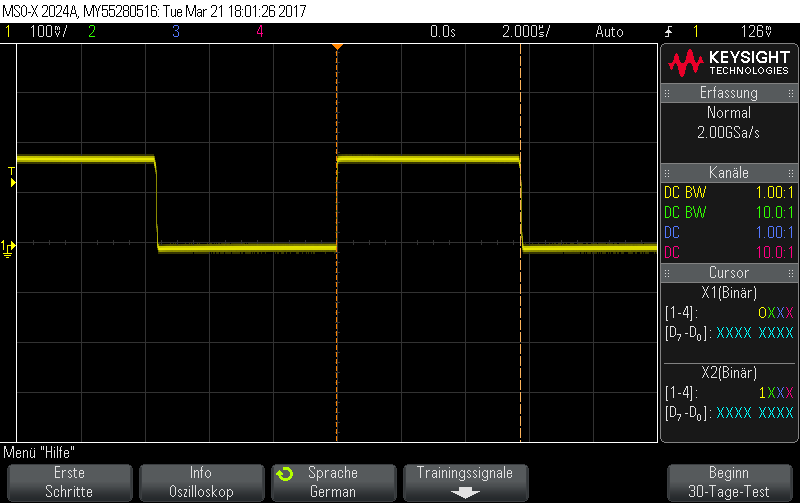
\includegraphics[width=\textwidth]{Images/1_1_MIPS}
	\caption[AnsteuerungsfrequenzLED]{Ansteuerungsfrequenz der LED}
	\label{image:AnsteuerungsfrequenzLED}
\end{figure}


\begin{lstlisting}[frame=htrbl, caption={Assembler Befehle zum toggeln}, label={lst:AssemblerToggle}]
//while(1){
// _LED200=!_LED200; //Toggle LED
00033E  8070A1     MOV LATB, W1
000340  201000     MOV #0x100, W0
000342  608000     AND W1, W0, W0
000344  A7F000     BTSC W0, #15
000346  EA0000     NEG W0, W0
000348  E90000     DEC W0, W0
00034A  DE004F     LSR W0, #15, W0
00034C  784000     MOV.B W0, W0
00034E  FB8000     ZE W0, W0
000350  600061     AND W0, #0x1, W0
000352  DD0048     SL W0, #8, W0
000354  8070A1     MOV LATB, W1
000356  A18001     BCLR W1, #8
000358  700001     IOR W0, W1, W0
00035A  8870A0     MOV W0, LATB
//}//while
00035C  37FFF0     BRA 0x33E
//return (EXIT_SUCCESS);  //never reached
//} //main()
\end{lstlisting}	
\newpage

\begin{figure}
	\centering
	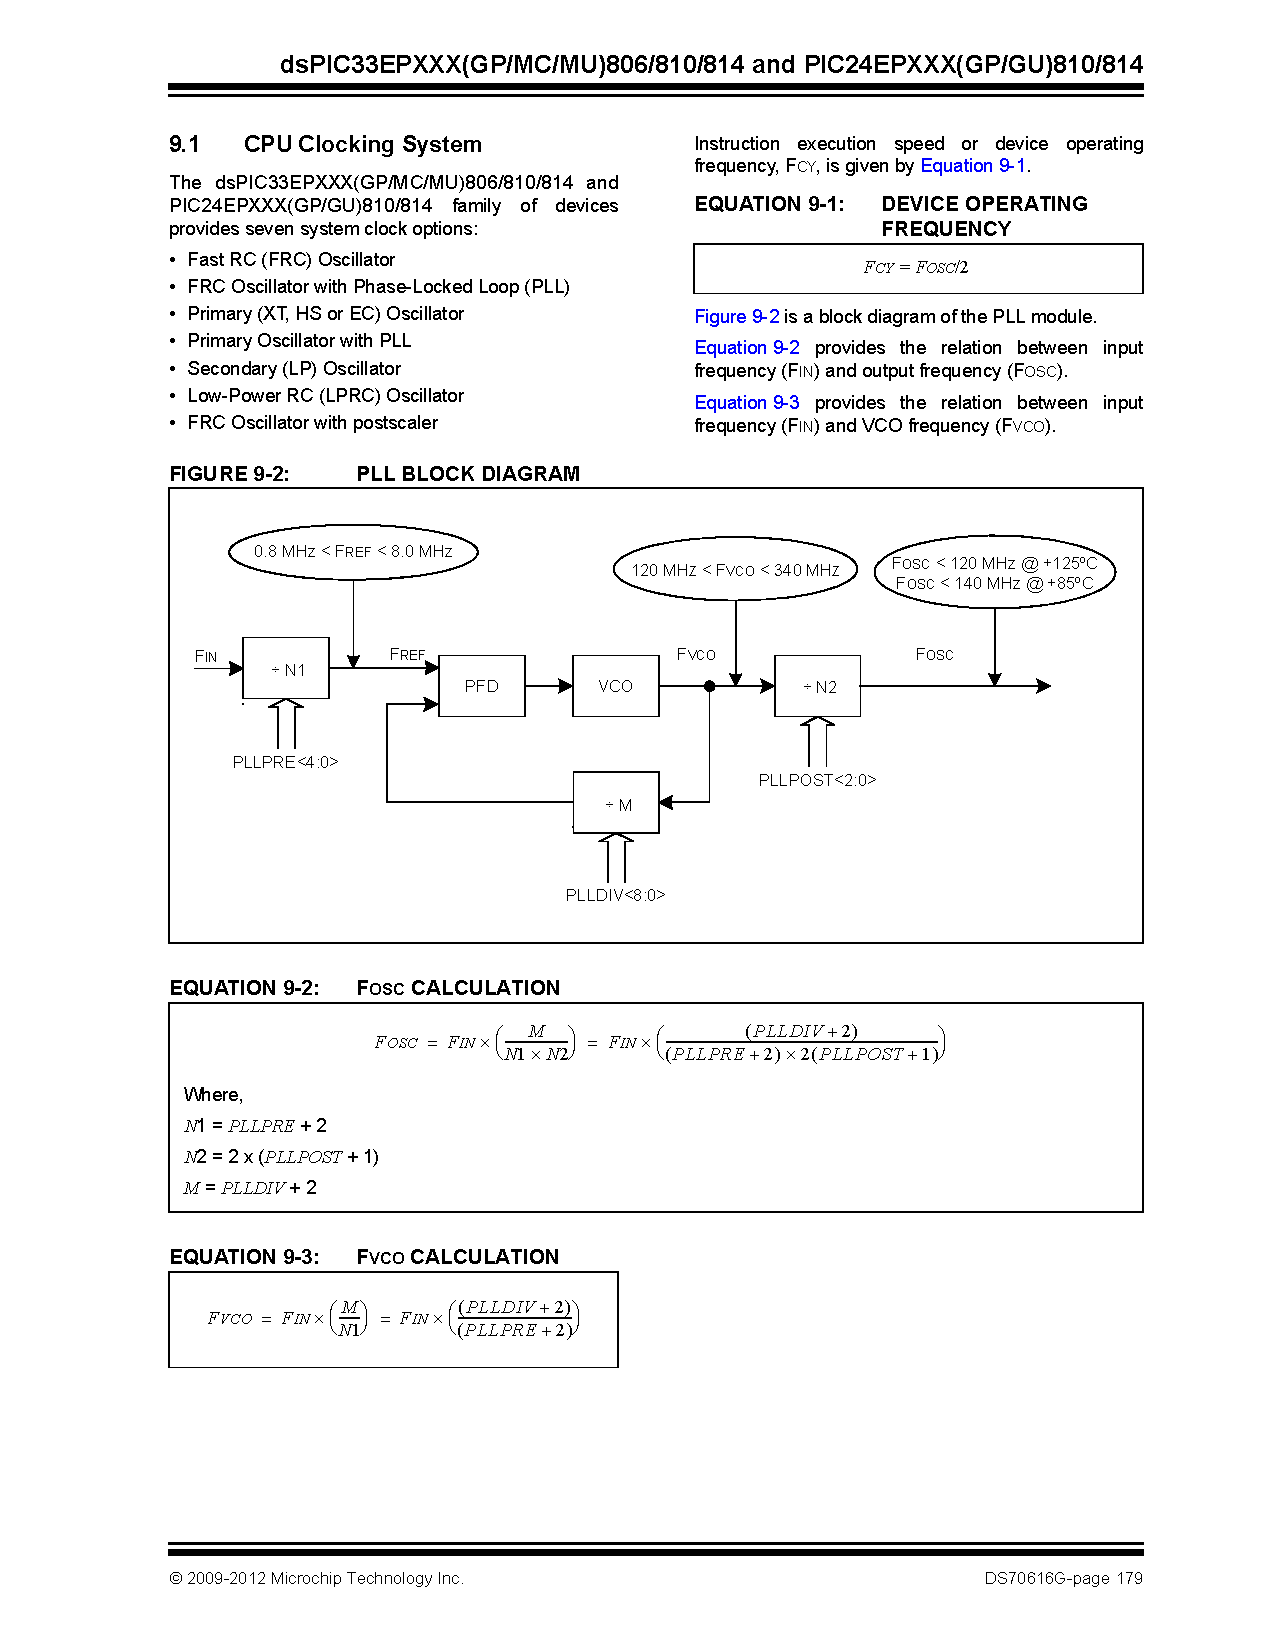
\includegraphics[width=\textwidth]{Images/CPUClockingSystem}
	\caption[CPU Blocking System]{CPU Clocking System mit PLL Block Diagramm}
	\label{image:CPUClockingSystem}
\end{figure}

\begin{figure}
	\centering
	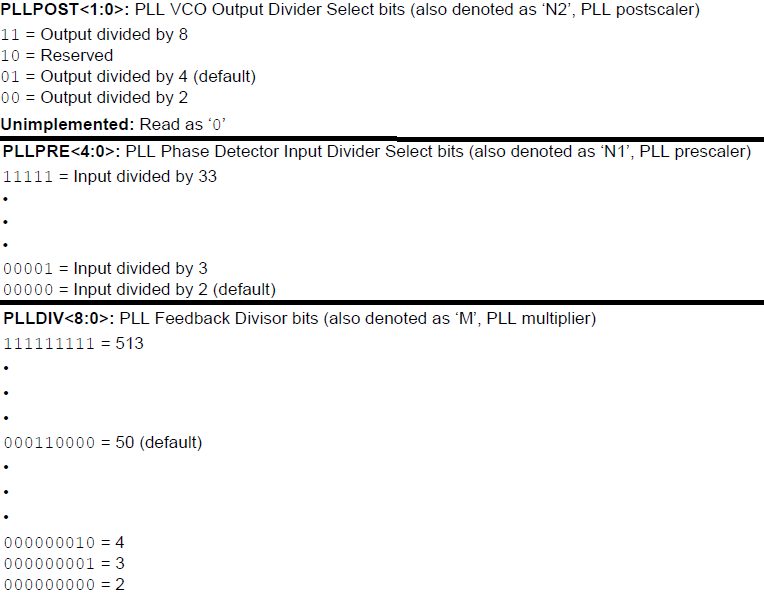
\includegraphics[width=\textwidth]{Images/PLLParameter}
	\caption[Wertebereich der PLL Parameter]{Wertebereich der PLL Parameter}
	\label{image:PLLParameter}
\end{figure}

\begin{figure}
	\centering
	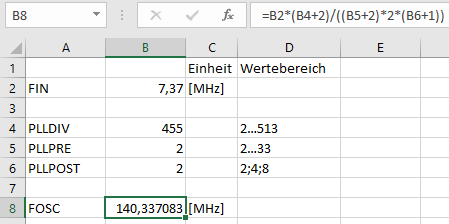
\includegraphics[width=0.95\textwidth]{Images/PLLParameterExcel}
	\caption[Berechnung der PLL Parameter in Excel]{PLL Parameter Excel}
	\label{image:PLLParameterExcel}
\end{figure}

\newpage
\begin{lstlisting}[frame=htrbl, caption={Code Example for Using PLL with 7.37 MHz Internal FRC}, label={lst:OscillatorSetup}]
// Select Internal FRC at POR
_FOSCSEL(FNOSC_PRIPLL); //Initial Oscillator: Primary Oscillator (XT, HS, EC) with PLL
_FOSC(POSCMD_HS);  //HS Crystal Oscillator Mode

int main()
{
// Configure PLL prescaler, PLL postscaler, PLL divisor
PLLFBD=455; // PLLDIV
CLKDIVbits.PLLPOST=2;
CLKDIVbits.PLLPRE=2;

// Wait for PLL to lock
while (OSCCONbits.LOCK!= 1);


while(1)
{
//endless loop
}

return 1; //never reached
}
\end{lstlisting}
